\section{Label-Swapping Algorithm}
\indent In this section, we present the \emph{label-swapping} algorithm which takes a graph $G$ and yields $G'$, a masking of $G$.This algorithm, as shown in figure \ref{fig:label-swap}, works by altering the original graph while maintaining the same $k-Neighborhood$. This is accomplished by partitioning the vertices of the graph into $adjacency$-$groups$.

\begin{figure}[htb]
	\begin{algorithmic}
		\renewcommand{\algorithmicrequire}{\textbf{Input:}}
		\renewcommand{\algorithmicensure}{\textbf{Output:}}
		\Require {List of Adjacency Groups $A$}
		\Ensure {Sorted List of Adjacency Groups $A'$}
		\State {Declare kTree $T$}
		\ForAll {$a \in A$}
			\State {Insert $a$ into a branch of $T$ sorting criteria}
		\EndFor
		\State {Extract sorted list of adjacency groups from $T$ as $A'$}
		\State \Return {$A'$}
	\end{algorithmic}
	\caption{Pseudocode for the kSort Algorithm.}
	\label{fig:kSort}
\end{figure}

\begin{figure}[htb]
	\begin{algorithmic}
		\renewcommand{\algorithmicrequire}{\textbf{Input:}}
		\renewcommand{\algorithmicensure}{\textbf{Output:}}
		\Require {Graph $G = (V, E)$, Integer $k$}
		\Ensure {Graph $G' = (V, E')$}
		\ForAll {$v \in V$}
			\State {calculate $N_k(v)$}
		\EndFor
		\State {Apply ksort algorithm to find adjacency groups}
		\ForAll {$A \in Adjacency Groups$}
			\State {find a valid swapping on $A$}
		\EndFor
		\ForAll {$(u,v) \in E$}
			\State {add edge $(Swap(u),Swap(v))$ to $E'$}
		\EndFor
		\State \Return {$G' = (V,E')$}
	\end{algorithmic}
	\caption{Pseudocode for the label-swapping algorithm.}
	\label{fig:label-swap}
\end{figure}

\indent The label-swapping algorithm, as shown in figure \ref{fig:label-swap} works by finding all maximal adjacency-groups and applying a random swapping to each one. The new graph formed by applying these swappings must have the same k-Neighborhood as the original graph (see Theorem 1); however, it may be possible to determine edges in the original graph from the new graph.
\\

\begin{figure}[ht]
  \centering
  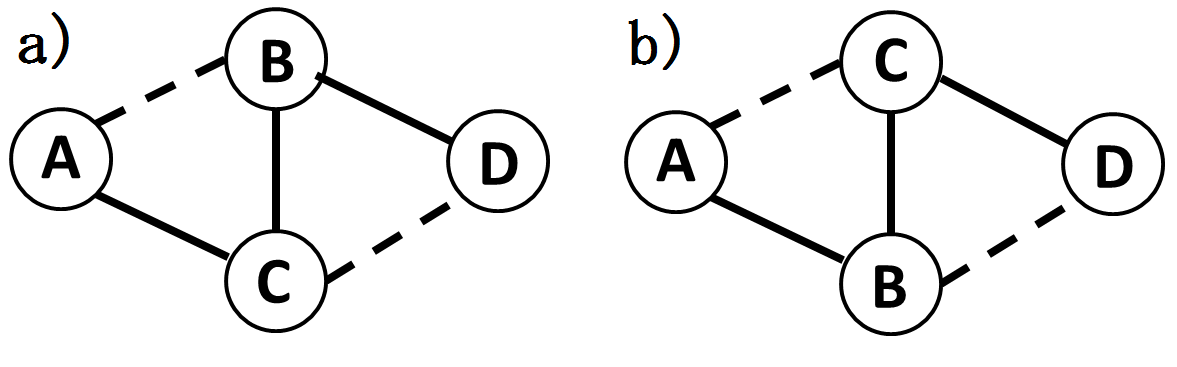
\includegraphics[scale=0.3 ]{Sample-Graph.png}
  \caption{In the above graphs, solid lines represent edges in the original graph and dotted lines represent edges that are only in the 2-Neighborhood graph (Note that all edges in the original graph are necessarily in the 2-Neighborhood graph). a)  The vertices B and C are in the same adjacency-group, while A and D are each in adjacency-groups of size 1. b) The result of applying a swapping to the adjacency group containing B and C, with the 2-Neighborhood graph remaining the same as the graph in (a).}
  \label{fig:sample graph}
\end{figure}




\begin{thm}  \emph{Applying a swapping to a graph, G, will yield a graph, G', with the same k-Neighborhood graph as G.}
\end{thm}
\begin{proof}
\noindent Let $G_k'$ be the k-Neighborhood graph of $G'$ and $G_k$ be the k-Neighborhood graph of $G$. Assume $G_k'$ is not equal to $G_k$. Then (i) $G_k'$ contains an edge not in $G_k$ or (ii) $G_k$ contains an edge not in $G_k'$.  \\
\indent i) Let $(u,v)$ be an edge in $G_k'$ that's not in $G_k$. Since $G'$ was formed by $swappings$ on $G$, $u$ must have some label $x$ and $v$ must have some label $y$ in $G$, where $x$ and $y$ were in the adjacency-groups of $u$ and $v$, respectively, and $(x,y)$ is in $G_k$. But, since $u$ and $x$ are in the same adjacency-group, and $(x,y)$ is in $G_k$, then $(u,y)$ must be in $G_k$. Since $y$ and $v$ are in the same adjacecy-group and $(u,y)$ is in $G_k$, then $(u,v)$ is in $G_k$, and our assumption that $G_k'$ has an edge that is not in $G_k$ must be false.\\
\indent 			ii) Let $(u,v)$ be an edge in $G_k$ that is not in $G_k'.$ Let the nodes labeled $x$ and $y$ in $G$ be given the labels $u$ and $v$, respectively, in $G'$. Therefore, $u$ and $x$ share an adjacency-group, as do $v$ and $y$.  Since $(u,v)$ is in $G_k$ and $u$ and $x$ share an adjacency-group, then $(x,v)$ is in $G_k$. Likewise, since $v$ and $y$ share an adjacency-group and $(x,v)$ is in $G_k$, then $(x,y)$ is in $G_k$. This implies that $(u,v)$ must be in $G_k'$. Therefore, our assumption that $G_k$ has an edge that is not in $G_k'$ is false. \\
\indent Because (i) and (ii) are false, we can conclude that $G_k$ equals $G_k'$.\\
\end{proof}
